导航最重要的技术就是
\textbf{SLAM(simultaneous localization and mapping,实时定位和建图技术)}简称SM(不是)。
先通过一个视频直观了解一下\url{https://www.bilibili.com/video/BV1tS4y1S7qE}
视频中随着机器人的移动,机器人的传感器获取到了环境信息,然后完成对博物馆地图的构建。
有小伙伴可能会问,只看到建图没看到定位呀。细心观察可以发现建图的过程中,其实一直都在计算机器人的位置。

该技术的基础就是定位。我们先来了解一下在ROS中如何表示定位信息。
在ROS中,我们使用tf树(transform tree)来表示物体(或者其他东西)之间的相对位置关系。
每个需要用到的东西(如车体,雷达,相机)都有一个以自身为原点的三维坐标系(frame)。
一个tf表示一个坐标系在另一个坐标系下的位姿信息(平移、旋转)。tf树的原理就是通过表示坐标系之间的关系来确定各个坐标系之间的相对位置。
常见的frame的约定俗成的名称有:
\begin{itemize}
\item /map:世界坐标系
\item /odom:里程计坐标系
\item /base\_link:小哨兵的坐标系
\item /camera\_link:相机坐标系
\item /laser\_link:激光雷达坐标
\item /imu\_link:IMU坐标系
\item ...
\end{itemize}

tf的主要信息包含父子节点(即两个坐标系,注意有父子关系,由父节点指向子节点)之间由xyz表示的平移关系和四元数表示的旋转关系。
多个父子节点的tf可以组成一个tf树,树的根节点一般是map,树的叶子节点一般是各个传感器的坐标系。
通过tf树可以算出任意两个节点之间的坐标关系(相对位置)。
\begin{figure}[H]
        \centering
        \includegraphics[width=0.8\textwidth]{./images/tf树.png}
        \caption{map到livox到livox\_192\_168\_1\_104的tf树}
\end{figure}
\begin{figure}[H]
        \centering
        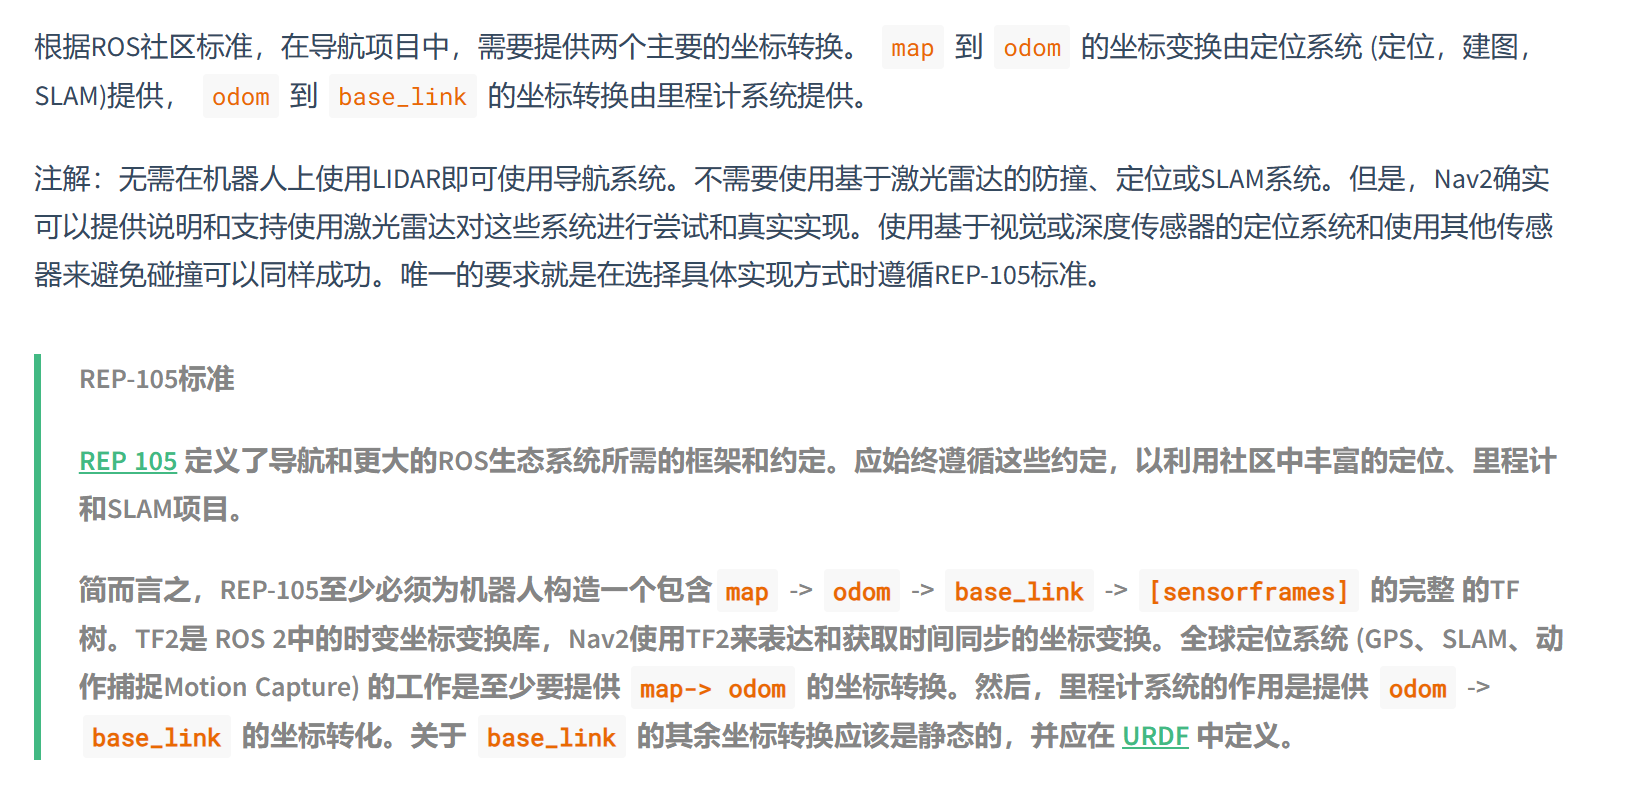
\includegraphics[width=1.0\textwidth]{./images/REP-105标准.png}
        \caption{REP-105标准}
\end{figure}
但是可怜的小哨兵并没有GPS直接定位。
所以他只能用其他的定位技术,比如激光雷达、IMU、里程计、视觉相机等。

\subsubsection{ 激光雷达定位}
先简单介绍一下激光雷达的工作原理:激光雷达的工作原理是通过发射一束激光,然后接收到反射回来的信号,通过解码,得到反射点的坐标,根据反射光的强弱还能获得强度信息。

激光雷达定位主要分为四步:
\begin{enumerate}
\item 所有定位方法开始,都要先要有一张已有的地图,地图上记录了各个障碍物的位置、大小、置信度等信息。将地图上的某一点设为原点,以原点为中心展开的坐标系为map坐标系。
\item 激光雷达扫描四周环境,得到一张激光雷达“视野内”的地图,上面记载了周围的障碍物信息(更多细节将在下一节详细介绍)
\item 将这张地图与已有的地图进行对比匹配,得到雷达最可能存在的位置,将该位置与map坐标系之间的相对位置变化记为map与ladar之间的tf。
\item 结合laser与baselink之间的tf(一般是提前固定写好的,由雷达固定在车体的位置和朝向决定),得到baselink与map之间的相对位置变化,即得到小哨兵在map坐标系下的位置。
\end{enumerate}
其中从匹配方式大体可分为两种:二维和三维匹配。
\begin{itemize}

\item 三维匹配:直接将扫描到的点云与之前存储的点云匹配,定位更准确,但是匹配速度慢(如ICP,NDT匹配算法)。常会用到kd-tree,oct-tree等数据结构加速匹配。
\item 二维匹配:将三维的点云信息按一定规则压缩到二维(二向箔),获得附近的实时的二维地图,与已有的地图进行匹配(如AMCL算法)。
                地图为栅格地图。
\end{itemize}
按照匹配对象来分,也可以分为两种:全局匹配和局部匹配。
\begin{itemize}
        \item 局部匹配:一般与先前一小段时间内的储存的点云或者栅格地图进行匹配,获得相对移动,是一种动态的匹配。
        因为要防止匹配目标过大,耗时太久,导致实时性不佳(局部路径规划对实时性需求较高),所以需要将较久之前扫描到的点云,或者距离较远的点云从kdtree之类的数据结构中清理掉。
        \item 全局匹配:将激光雷达的扫描信息与整个地图进行匹配,得到小哨兵的位置。一般用于重定位,即小哨兵迷失了方向的时候
                (如刚刚上电不知道自己在哪;被狠狠地创飞了,定位可能歪了;被神秘的力量干扰,导致进入恢复行为树;刚从恢复行为里出来,与定位系统失联许久……),将原先的tf清除,重新进行定位。
\end{itemize}
运动过程中多用动态的匹配,以便较快的更新定位,提高实时性。与整张全局地图的匹配,一般在特定情况下(如刚开机上电不知道自己在哪的时候;定位可能出现偏差的情况;或者执行完恢复行为之后。也可以时不时重定位一下,上赛季就是这么干的,效果好像不太行QAQ)才进行,又叫重定位,即直接清零更新baselink和map之间的tf。
\subsubsection{ 里程计,IMU定位}
里程计定位较为简单,直接获取机器人各个方向运动的里程,加在map坐标系下的位置即为小哨兵的位置。
IMU,即惯性测量单元,可以测量各方向的角速度和线加速度,通过积分,获得类似里程计的数据,加在map坐标系下的位置即为小哨兵的位置。
这两个方法一般电控端就可以独立完成,纯电控的机器人常用。

\subsubsection{ 视觉定位}
视觉定位也是近年来较为流行的SLAM技术,它与激光雷达定位类似,但他获取的特征信息在相同情况下比激光雷达多。
它通过提取图像中的特征点(一般是角点),与原先存储的地图里的特征点对比匹配,计算出相机的相对位移,累加后得到小哨兵在map坐标系的坐标变换。

\subsubsection{ 多传感器融合}
以上各个定位方法都有自己的局限性:
\begin{itemize}
\item imu,里程计定位:由于IMU和里程计对运动(速度,加速度)测量的精度较高,定位较为准确。但由于其本身稳定性较差,易受干扰(如IMU受热噪声干扰的零漂,轮式里程计打滑等情况);
        且他们都是“开环”的测量方式,一旦出现意外情况(比如受干扰,或者某些情况下超过其测量范围(比如被别的机器人肘了一下,瞬时加速度太大IMU测量不了)),
        测量的位置歪掉了,就再也回不来了,因为没法校正。
\item 视觉定位:视觉定位的精度较低,且受相机的分辨率、光照、遮挡等因素影响较大。且对需要物体纹理较多效果才比较好。
\item 雷达定位:激光雷达只能获取深度信息,这会导致在一些特殊情况中定位失效。
        如雷达在非常长的两堵一模一样的墙之间前进,虽然车在前进,但在雷达的视野里,左右离墙的距离不变,而前后因为超出探测距离所以数据也不变,他就以为自己没有运动了;
        又如雷达在一个一个正方形房间的正中心,你趁雷达不注意(即在两次雷达扫描的间隔之间),把他旋转90度。在雷达的视野里,前后左右的障碍物与之前的完全相同,所以他会以为自己没旋转。
\end{itemize}
为了解决这些问题,人们将多种传感器的数据融合在一起得到更准确定位方法。

基本原理是通过前后数据之间对比得出机器人位置的变化。
然后回环检测,判断机器人是否到达之前到过的位置,可以解决位置估计误差问题,建图时可以纠正地图误差。

最常见的融合方法(也是我们现在使用的方法)是激光雷达和里程计的融合。
我们新建一个节点odom,他作为map的子节点,作为base\_link的父节点。
里程计提供 odom -> base\_link 的tf。
里程计可以来自许多数据源,包括激光雷达、车轮编码器、VIO和IMU。
里程计的目标是提供基于机器人运动的平滑和连续的局部坐标系。
这样平滑输出就可用于精确运动的航行位置推算和在全局位置更新之间准确地更新机器人的位置。

而雷达重定位输出map到odom的tf作为校正数值记录。
全局定位系统会相对全局坐标的坐标变换进行更新,以解决里程计的漂移问题。

这样,小哨兵的位置就通过激光雷达和里程计 fusion 的方式得到。

其他的融合方法还有:激光雷达与视觉融合,将点云与图像匹配,使点云除了位置信息外,还能拥有颜色等信息。
\begin{figure}[H]
        \centering
        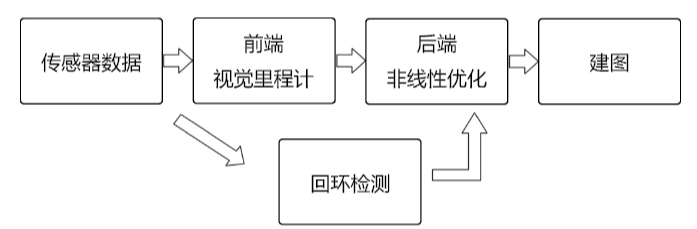
\includegraphics[width=0.8\textwidth]{./images/经典视觉SLAM结构.png}
        \caption{经典视觉SLAM结构}
\end{figure}

从算法的对数据的处理方式上看,目前常用的SLAM开源算法可以分为两类

1.基于滤波:
比如扩展卡尔曼滤波(EKF: Extended Kalman Filter)、粒子滤波(PF: Particle Filter)等。
ROS中的gmapping、hector\_slam算法都是基于滤波实现的。
我们使用的point-lio也使用了流形扩展卡尔曼滤波。

2.基于图优化,先通过传感器进行构图,然后对图进行优化。

